%% abtex2-modelo-relatorio-tecnico.tex, v<VERSION> laurocesar
%% Copyright 2012-<COPYRIGHT_YEAR> by abnTeX2 group at http://www.abntex.net.br/
%%
%% This work may be distributed and/or modified under the
%% conditions of the LaTeX Project Public License, either version 1.3
%% of this license or (at your option) any later version.
%% The latest version of this license is in
%%   http://www.latex-project.org/lppl.txt
%% and version 1.3 or later is part of all distributions of LaTeX
%% version 2005/12/01 or later.
%%
%% This work has the LPPL maintenance status `maintained'.
%%
%% The Current Maintainer of this work is the abnTeX2 team, led
%% by Lauro César Araujo. Further information are available on
%% http://www.abntex.net.br/
%%
%% This work consists of the files abntex2-modelo-relatorio-tecnico.tex,
%% abntex2-modelo-include-comandos and abntex2-modelo-references.bib
%%

% ------------------------------------------------------------------------
% ------------------------------------------------------------------------
% abnTeX2: Modelo de Relatório Técnico/Acadêmico em conformidade com
% ABNT NBR 10719:2015 Informação e documentação - Relatório técnico e/ou
% científico - Apresentação
% ------------------------------------------------------------------------
% ------------------------------------------------------------------------

\documentclass[
	% -- opções da classe memoir --
	12pt,				% tamanho da fonte
	openright,			% capítulos começam em pág ímpar (insere página vazia caso preciso)
	twoside,			% para impressão em recto e verso. Oposto a oneside
	a4paper,			% tamanho do papel.
	% -- opções da classe abntex2 --
	%chapter=TITLE,		% títulos de capítulos convertidos em letras maiúsculas
	%section=TITLE,		% títulos de seções convertidos em letras maiúsculas
	%subsection=TITLE,	% títulos de subseções convertidos em letras maiúsculas
	%subsubsection=TITLE,% títulos de subsubseções convertidos em letras maiúsculas
	% -- opções do pacote babel --
	english,			% idioma adicional para hifenização
	french,				% idioma adicional para hifenização
	spanish,			% idioma adicional para hifenização
	brazil,				% o último idioma é o principal do documento
	]{abntex2}


% ---
% PACOTES
% --- How do I remove blank pages coming between two chapters in Appendix?
%\documentclass[oneside]{book}

% ---
% Pacotes fundamentais
% ---
\usepackage{lmodern}			% Usa a fonte Latin Modern
\usepackage[T1]{fontenc}		% Selecao de codigos de fonte.
\usepackage[utf8]{inputenc}		% Codificacao do documento (conversão automática dos acentos)
\usepackage{indentfirst}		% Indenta o primeiro parágrafo de cada seção.
\usepackage{color}				% Controle das cores
\usepackage{graphicx}			% Inclusão de gráficos
\usepackage{microtype} 			% para melhorias de justificação
% ---
\usepackage{graphicx} % Required for including pictures
\graphicspath{{img/}} % Specifies the directory where pictures are stored
% ---
% Pacotes adicionais, usados no anexo do modelo de folha de identificação
% ---
\usepackage{multicol}
\usepackage{multirow}
% ---
\usepackage{amssymb}

% ---
% Pacotes adicionais, usados apenas no âmbito do Modelo Canônico do abnteX2
% ---
\usepackage{lipsum}				% para geração de dummy text
% ---

% ---
% Pacotes de citações
% ---
\usepackage[brazilian,hyperpageref]{backref}	 % Paginas com as citações na bibl
\usepackage[alf]{abntex2cite}	% Citações padrão ABNT
\usepackage{verbatim}
\usepackage{enumitem}


% ---
% CONFIGURAÇÕES DE PACOTES
% ---
\usepackage{afterpage}
\usepackage{emptypage}


% ---
% Configurações do pacote backref
% Usado sem a opção hyperpageref de backref
\renewcommand{\backrefpagesname}{Citado na(s) página(s):~}
% Texto padrão antes do número das páginas
\renewcommand{\backref}{}
% Define os textos da citação
\renewcommand*{\backrefalt}[4]{
	\ifcase #1 %
		Nenhuma citação no texto.%
	\or
		Citado na página #2.%
	\else
		Citado #1 vezes nas páginas #2.%
	\fi}%
% ---
% Informações de dados para CAPA e FOLHA DE ROSTO
% ---
\titulo{Linguagens Formais Avaliação 4\\ Relatório Técnico e/ou Científico}
\autor{Daniel Terra Gomes, José Lucio Azevedo}
\local{Campos dos Goytacazes, RJ}
\data{20, Junho de 2022, v1.0.0}
\instituicao{%
Universidade Estadual do Norte Fluminense Darcy Ribeiro - UENF
  \par
  CIÊNCIA DA COMPUTAÇÃO
  \par
  INF01117 - Linguagens Formais}
\tipotrabalho{Relatório técnico}
% O preambulo deve conter o tipo do trabalho, o objetivo,
% o nome da instituição e a área de concentração
\preambulo{Relatório técnico da Avaliação 4 apresentado ao Curso de Ciência da Computação da Universidade Estadual do Norte Fluminense Darcy Ribeiro, como requisito avaliativo da disciplina.}
% ---

% ---
% Configurações de aparência do PDF final

% alterando o aspecto da cor azul
\definecolor{blue}{RGB}{41,5,195}

% informações do PDF
\makeatletter
\hypersetup{
     	%pagebackref=true,
		pdftitle={\@title},
		pdfauthor={\@author},
    	pdfsubject={\imprimirpreambulo},
	    pdfcreator={LaTeX with abnTeX2},
		pdfkeywords={abnt}{latex}{abntex}{abntex2}{relatório técnico},
		colorlinks=true,       		% false: boxed links; true: colored links
    	linkcolor=blue,          	% color of internal links
    	citecolor=blue,        		% color of links to bibliography
    	filecolor=magenta,      		% color of file links
		urlcolor=blue,
		bookmarksdepth=4
}
\makeatother
% ---

% ---
% Espaçamentos entre linhas e parágrafos
% ---

% O tamanho do parágrafo é dado por:
\setlength{\parindent}{1.3cm}

% Controle do espaçamento entre um parágrafo e outro:
\setlength{\parskip}{0.2cm}  % tente também \onelineskip

% ---
% compila o indice
% ---
\makeindex
% ---

% ----
% Início do documento
% ----
\begin{document}
% Seleciona o idioma do documento (conforme pacotes do babel)
%\selectlanguage{english}
\selectlanguage{brazil}
% Retira espaço extra obsoleto entre as frases.
\frenchspacing
% ----------------------------------------------------------
% ELEMENTOS PRÉ-TEXTUAIS
% ----------------------------------------------------------
\pretextual
% ---
% Capa
% ---
\imprimircapa

% ---
% ---
% Folha de rosto
% (o * indica que haverá a ficha bibliográfica)
% ---
\imprimirfolhaderosto*
% ---
% ---
% Anverso da folha de rosto:
% ---
% ---
% RESUMO
% ---
% resumo na língua vernácula (obrigatório)

% ---
% ---
% inserir lista de ilustrações
% ---
\pdfbookmark[0]{\listfigurename}{lof}
\listoffigures*
\cleardoublepage
% ---

% ---
% inserir lista de tabelas
% ---
%\pdfbookmark[0]{\listtablename}{lot}
%\listoftables*
%\cleardoublepage
% ---

% ---
% inserir lista de abreviaturas e siglas
% ---
%\begin{siglas}
%  \item[ABNT] Associação Brasileira de Normas Técnicas
%  \item[abnTeX] ABsurdas Normas para TeX
%\end{siglas}
% ---

% ---
% inserir lista de símbolos
% ---
%\begin{simbolos}
%  \item[$ \Gamma $] Letra grega Gama
%  \item[$ \Lambda $] Lambda
%  \item[$ \zeta $] Letra grega minúscula zeta
%  \item[$ \in $] Pertence
%\end{simbolos}
% ---

% ---
% inserir o sumario
% ---
%\pdfbookmark[0]{\contentsname}{toc}
%\tableofcontents*
%\cleardoublepage
% ---


% ----------------------------------------------------------
% ELEMENTOS TEXTUAIS
% ----------------------------------------------------------
\textual

% ----------------------------------------------------------
% Introdução (exemplo de capítulo sem numeração, mas presente no Sumário)
% ----------------------------------------------------------
\chapter*[Introdução]{Introdução}
\addcontentsline{toc}{chapter}{Introdução}
As atividades propostas para esse relatório se iniciam por perguntas sobre \emph{Autômato de Pilha}. Sendo a primeira pergunta \ref{77} relacionada a projetar um autômato de pilha para aceitar uma linguagem. Esse tipo de autômatos são máquinas de estado finito não determinísticas aumentadas com memória adicional na forma de uma pilha, e é por isso que o termo “pushdown” (Autômato de Pilha) é usado, à medida que os elementos são empurrados para baixo na pilha. Os autômatos de empilhamento são modelos computacionais – máquinas teóricas semelhantes a computadores – que podem fazer mais do que uma máquina de estados finitos, mas menos do que uma máquina de Turing \footnote{\url{https://brilliant.org/wiki/pushdown-automata/}}.

Formalmente, um autômato de pilha é uma máquina não determinística definida pela 7-tupla $(Q, \Sigma, \Gamma,  \delta, q0 , Z0 , F)$, onde

  \textsf{Q} é um conjunto finito de estados;

  \textsf{$\Sigma$} é um alfabeto;

  \textsf{$\Gamma$} é o alfabeto da pilha de símbolos que podem ser colocados na pilha;

  \textsf{$\delta$}:$ Q \times \Sigma\epsilon \times \Gamma \epsilon \rightarrow (Q \times \Gamma*)$ é a função transição, onde nenhuma tupla é mapeada para um conjunto infinito;

  \textsf{q0}$ \in$ Q é o estado inicial;

  \textsf{Z0} $\in \Gamma$ é o símbolo inicial da pilha e;

  \textsf{F} $\subseteq $Q é o conjunto de estados de aceitação.

O autômato é aceito se terminar em um estado de aceitação sem nenhuma entrada restante \footnote{\url{https://web.stanford.edu/class/archive/cs/cs103/cs103.1132/lectures/17/Small17.pdf}}.


Em seguida, se é apresentado um exercício sobre  \emph{Máquina de Turing} \ref{2} se pede para considerar uma Máquina de Turing que aceita um alfabeto, com uma fita com um funcionamento específico.
Essas máquinas de Turing, foram descritas pela primeira vez por Alan Turing em Turing 1936-7, são dispositivos computacionais abstratos simples destinados a ajudar a investigar a extensão e as limitações do que pode ser computado \footnote{\url{https://plato.stanford.edu/entries/turing-machine/}}. Essa Máquina é um dispositivo de aceitação que aceita as linguagens (conjunto recursivamente enumerável) geradas por gramáticas do tipo 0 (As gramáticas do tipo 0 incluem todas as gramáticas formais. Eles geram exatamente todas as linguagens que podem ser reconhecidas por uma máquina de Turing. Essas linguagens também são conhecidas como linguagens recursivamente enumeráveis ou Turing-reconhecíveis\footnote{\url{https://www.geeksforgeeks.org/chomsky-hierarchy-in-theory-of-computation/}}).
Máquinas de Turing é um modelo matemático que consiste em uma fita de comprimento infinito dividida em células nas quais a entrada é fornecida. Consiste em um cabeçote que lê a fita de entrada. Um registrador de estado armazena o estado da máquina de Turing. Depois de ler um símbolo de entrada, ele é substituído por outro símbolo, seu estado interno é alterado e ele se move de uma célula para a direita ou para a esquerda. Se a Máquinas de Turing  atingir o estado final, a string de entrada é aceita, caso contrário, rejeitada \footnote{\url{https://www.tutorialspoint.com/automata_theory}}.

Uma Máquinas de Turing pode ser formalmente descrita como uma 7-tupla $(Q, X, \Sigma, \delta,  q0, B, F)$, onde

    \textsf{Q} é um conjunto finito de estados;

    \textsf{X} é o alfabeto da fita;

    \textsf{$\Sigma$} é o alfabeto de entrada;

    \textsf{$\delta$} é uma função de transição; $\delta: Q \times X \rightarrow Q \times X \times {Left_shift, Right_shift}$;

    \textsf{q0} é o estado inicial;

    \textsf{B} é o símbolo em branco;

    \textsf{F} é o conjunto dos estados finais.\\


Por último, se é solicitado a resolução de exercício sobre uma \emph{gramática} \ref{7}, e a partir dela determinar suas características, derivações, e linguagem.

Todas as atividades apresentadas nesse relatório, também, seguiram o material teórico disponibilizado pelo Prof. Daniel Lucrédio \cite{lucredio} \footnote{\url{https://www.youtube.com/playlist?list=PLaPmgS59eMSGBPhHwyDLUzFrtTsc2yHJt}}.


% ----------------------------------------------------------
% PARTE - preparação da pesquisa
% ----------------------------------------------------------
\part{Apresentação das atividades}
\chapter{Perguntas}
\section{Autômato de pilha}
\begin{figure}[h]
  \begin{center}
    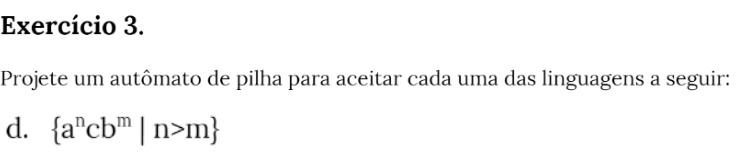
\includegraphics[width=15cm]{av4-ex3.png} \\
    \caption{Projete um autômato de pilha} \label{77}

  \end{center}
 \end{figure}


 \section{Máquina de Turing}
  \begin{figure}[h]
   \begin{center}
     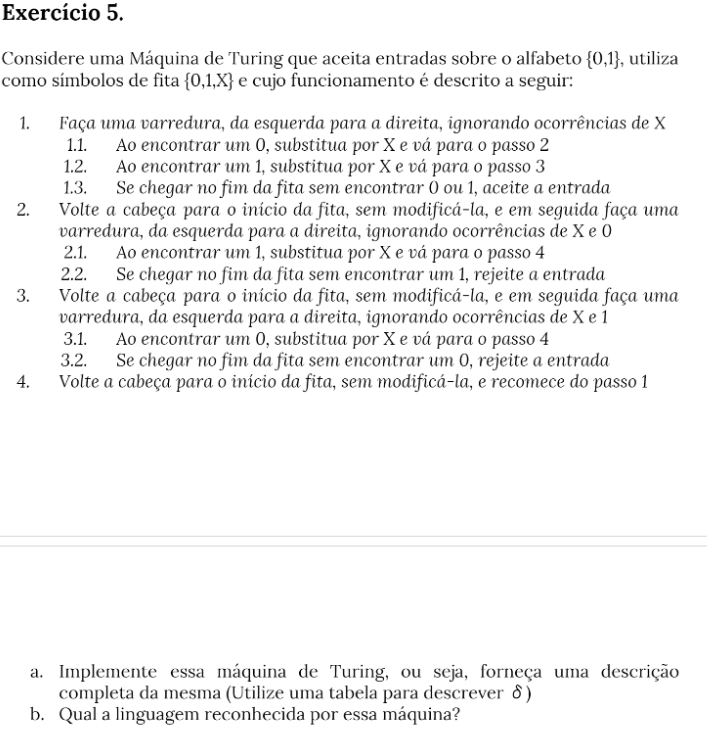
\includegraphics[width=11cm]{av4-ex5.png} \\
     \caption{Máquina de Turing sobre um alfabeto} \label{2}

   \end{center}
  \end{figure}

 \section{A partir da Gramática determine}
  \begin{figure}[h]
   \begin{center}
     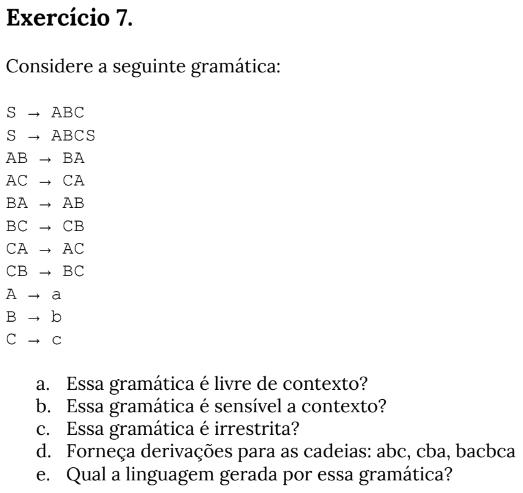
\includegraphics[width=12cm]{av4-ex7.png} \\
     \caption{Gramática} \label{7}

   \end{center}
  \end{figure}

% ----------------------------------------------------------
% Capitulo com exemplos de comandos inseridos de arquivo extern


% ----------------------------------------------------------
% Parte de resultados
% ----------------------------------------------------------
\part{Resultados}
% ---
% Capitulo de revisão de literatura
% ---
\chapter{Respostas}

\section{Apresentação dos resultados autômato de pilha}

\begin{figure}[h]
  \begin{center}
    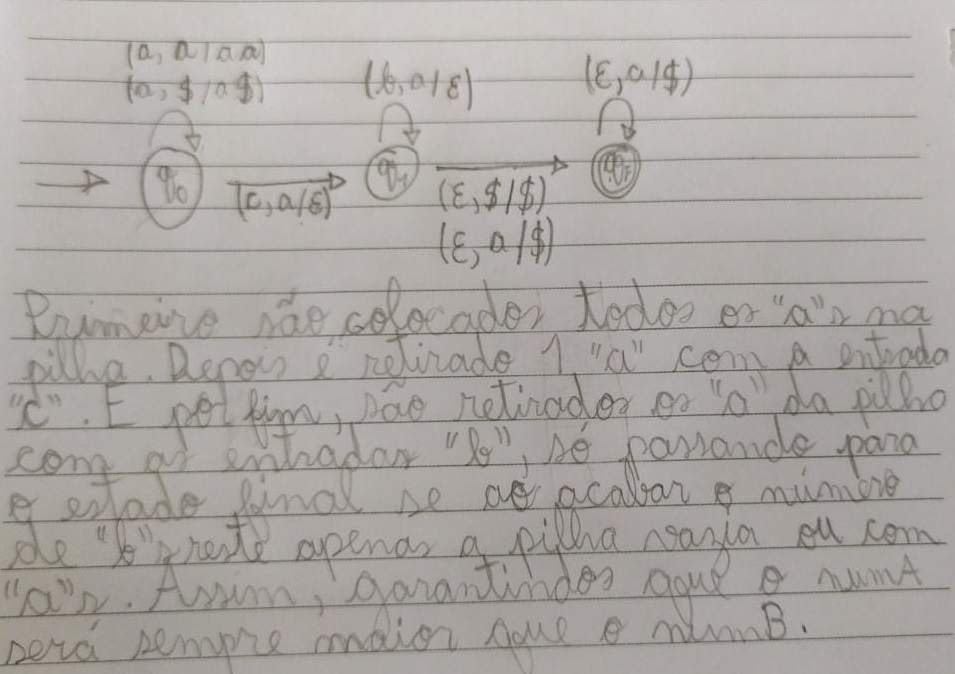
\includegraphics[width=12cm]{ex3} \\
    \caption{autômato de pilha} \label{r7}

  \end{center}
 \end{figure}



\section{Apresentação dos resultados Máquina de Turing}

\begin{figure}[h]
  \begin{center}
    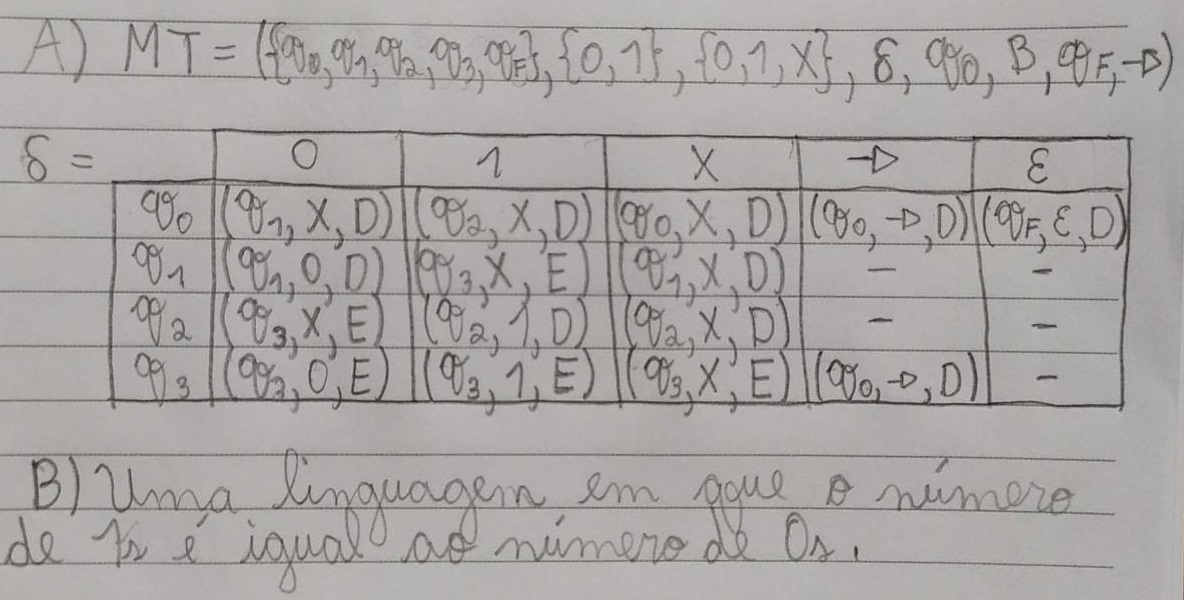
\includegraphics[width=12cm]{ex5} \\
    \caption{Máquina de Turing} \label{r2}

  \end{center}
\end{figure}

\begin{figure}[h]
  \begin{center}
    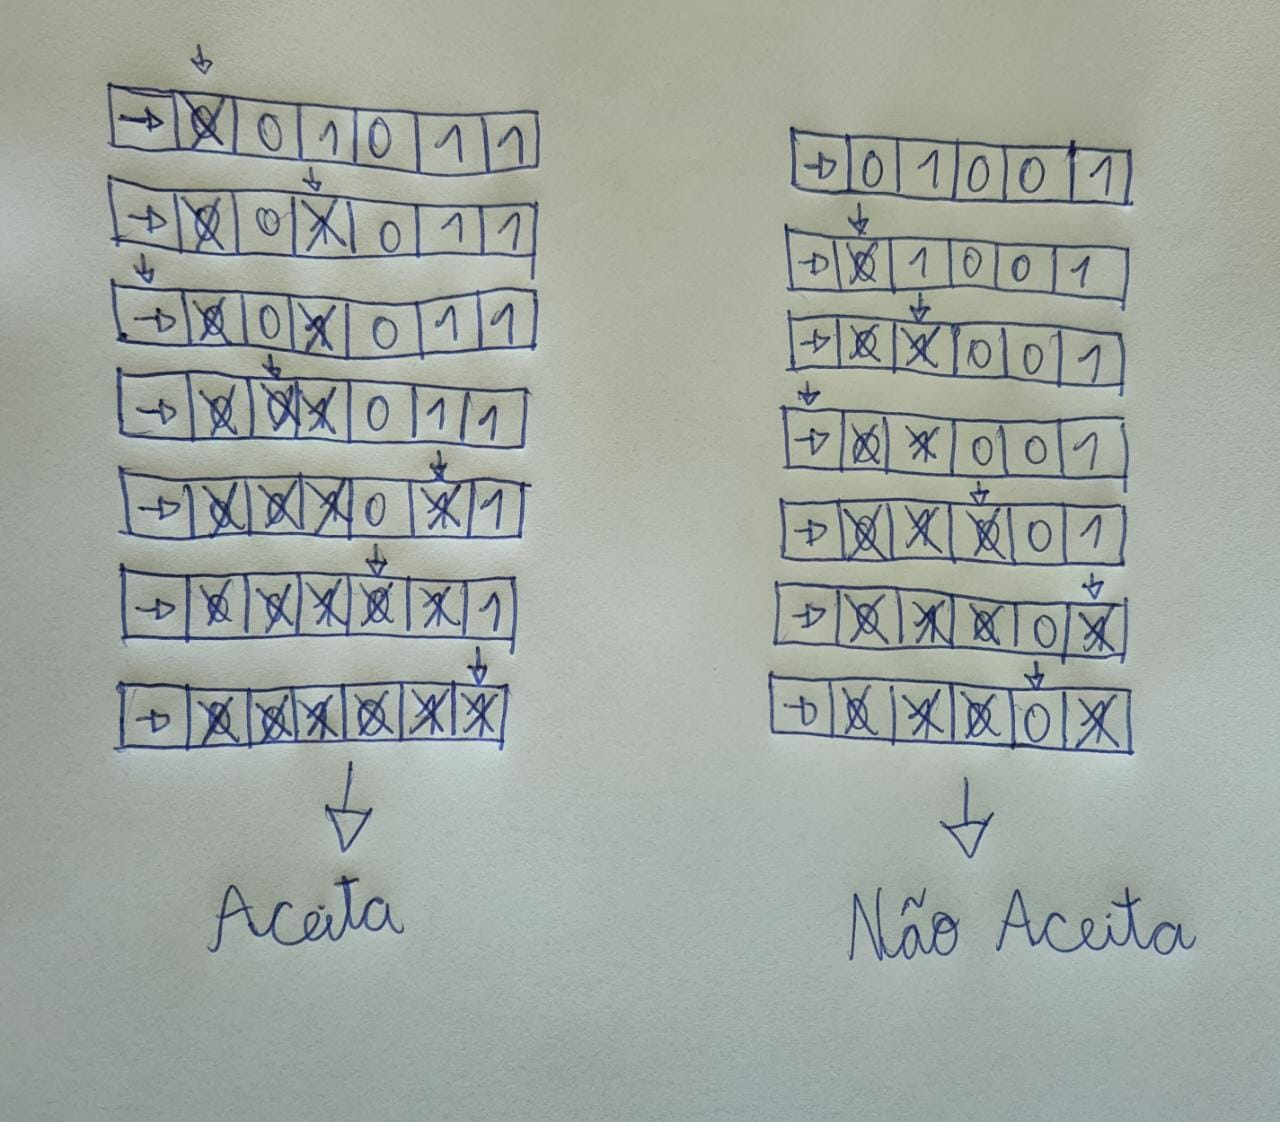
\includegraphics[width=10cm]{ex5-1.jpeg} \\
    \caption{Máquina de Turing} \label{r2-1}

  \end{center}
\end{figure}

\section{Apresentação dos resultados Gramática}

\begin{enumerate}[label=\alph*.]
  \item Sim, do lado esquerdo da produção deve, sempre ocorrer um e apenas um não terminal e do lado direito pode ocorrer qualquer coisa exceto a sentença vazia.

  \item Sim, pois a gramatica tem os lados esquerdo e direito de qualquer regra de produção podendo ser cercados por um contexto de símbolo terminal e símbolo não-terminal.
  Em Teoria da computação uma gramática sensível ao contexto (GSC), também conhecida como Tipo 1 da Hierarquia de Chomsky.

  \item Não, pois não é capaz de gerar linguagens recursivamente enumeráveis. São um tipo de linguagem formal que também é chamada de linguagem Turing-reconhecível. Também é conhecida como tipo-0 na hierarquia de Chomsky das linguagens formais.\\

  \item Derivação para \emph{abc}:

    $S  \rightarrow ABC$

    $A  \rightarrow aBC$

$B  \rightarrow abC$

$C  \rightarrow abc$

Derivação para \emph{cba}:

$S  \rightarrow ABC$

$AB  \rightarrow BAC$

$AC  \rightarrow BCA$

$BC  \rightarrow CBA$

$A  \rightarrow CBa$

$B  \rightarrow Cba$

$C  \rightarrow cba$

Derivação para \emph{bacbca}:

$S  \rightarrow ABCS$

$S  \rightarrow ABCABC$

$AB  \rightarrow BACABC$

$AB  \rightarrow BACBAC$

$AC  \rightarrow BACBCA$

$A  \rightarrow BaCBCA$

$B  \rightarrow baCBCA$

$C  \rightarrow bacBCA$

$A  \rightarrow BacBCa$

$B  \rightarrow bacbCa$

$C  \rightarrow bacbca$ \\


\item Seja \emph{L} a linguagem gerada acima e w uma palavra pertencente a \emph{L}, então w é uma palavra formada por qualquer combinação de \emph{a,b,c} onde a quantidade de símbolos \emph{a = b = c}.

\end{enumerate}
% ---

% ---
% Finaliza a parte no bookmark do PDF
% para que se inicie o bookmark na raiz
% e adiciona espaço de parte no Sumário
% ---


% ---
% Conclusão
% ---
\chapter{Conclusão}
% ---

Desse modo, podemos concluir que foram encontradas todas as soluções desejadas das atividades propostas.

% ----------------------------------------------------------
% ELEMENTOS PÓS-TEXTUAIS
% ----------------------------------------------------------
\postextual

% ----------------------------------------------------------
% Referências bibliográficas
% ----------------------------------------------------------
\bibliography{abntex2-modelo-references}

% ----------------------------------------------------------
% Glossário
% ----------------------------------------------------------
%
% Consulte o manual da classe abntex2 para orientações sobre o glossário.
%
%\glossary

% ----------------------------------------------------------
% Apêndices
% ----------------------------------------------------------
\begin{comment}
% ---
% Inicia os apêndices
% ---
\begin{apendicesenv}

% Imprime uma página indicando o início dos apêndices
\partapendices

% ----------------------------------------------------------
\chapter{Quisque libero justo}
% ----------------------------------------------------------

\lipsum[50]

% ----------------------------------------------------------
\chapter{Nullam elementum urna vel imperdiet sodales elit ipsum pharetra ligula
ac pretium ante justo a nulla curabitur tristique arcu eu metus}
% ----------------------------------------------------------
\lipsum[55-57]

\end{apendicesenv}
% ---


% ----------------------------------------------------------
% Anexos
% ----------------------------------------------------------

% ---
% Inicia os anexos
% ---
\begin{anexosenv}

% Imprime uma página indicando o início dos anexos
\partanexos

% ---
\chapter{Morbi ultrices rutrum lorem.}
% ---
\lipsum[30]

% ---
\chapter{Cras non urna sed feugiat cum sociis natoque penatibus et magnis dis
parturient montes nascetur ridiculus mus}
% ---

\lipsum[31]

% ---
\chapter{Fusce facilisis lacinia dui}
% ---

\lipsum[32]

\end{anexosenv}

%---------------------------------------------------------------------
% INDICE REMISSIVO
%---------------------------------------------------------------------

\phantompart

\printindex

%---------------------------------------------------------------------
% Formulário de Identificação (opcional)
%---------------------------------------------------------------------
\chapter*[Formulário de Identificação]{Formulário de Identificação}
\addcontentsline{toc}{chapter}{Exemplo de Formulário de Identificação}
\label{formulado-identificacao}

Exemplo de Formulário de Identificação, compatível com o Anexo A (informativo)
da ABNT NBR 10719:2015. Este formulário não é um anexo. Conforme definido na
norma, ele é o último elemento pós-textual e opcional do relatório.

\bigskip

\begin{tabular}{|p{9cm}|p{5cm}|}
\hline
\multicolumn{2}{|c|}{\textbf{\large Dados do Relatório Técnico e/ou científico}}\\
\hline
\multirow{4}{10cm}[24pt]{Título e subtítulo}& Classificação de segurança\\
                   & \\
                   \cline{2-2}
                   & No.\\
                   & \\

\hline
Tipo de relatório & Data\\
\hline
Título do projeto/programa/plano & No.\\
\hline
\multicolumn{2}{|l|}{Autor(es)} \\
\hline
\multicolumn{2}{|l|}{Instituição executora e endereço completo} \\
\hline
\multicolumn{2}{|l|}{Instituição patrocinadora e endereço completo} \\
\hline
\multicolumn{2}{|l|}{Resumo}\\[3cm]
\hline
\multicolumn{2}{|l|}{Palavras-chave/descritores}\\
\hline
\multicolumn{2}{|l|}{
Edição \hfill No. de páginas \hfill No. do volume \hfill Nº de classificação \phantom{XXXX}} \\
\hline
\multicolumn{2}{|l|}{
ISSN \hfill \hfill Tiragem \hfill Preço \phantom{XXXXXXXX}} \\
\hline
\multicolumn{2}{|l|}{Distribuidor} \\
\hline
\multicolumn{2}{|l|}{Observações/notas}\\[3cm]
\hline
\end{tabular}
\end{comment}
\end{document}
